% sage_latex_guidelines.tex V1.01, 11 June 2015

\documentclass[Afour,sagev,times,doublespace]{sagej}

\usepackage{moreverb,url}

\usepackage[colorlinks,bookmarksopen,bookmarksnumbered,citecolor=red,urlcolor=red]{hyperref}

\usepackage{epstopdf}

\newcommand\BibTeX{{\rmfamily B\kern-.05em \textsc{i\kern-.025em b}\kern-.08em
T\kern-.1667em\lower.7ex\hbox{E}\kern-.125emX}}

\def\volumeyear{2016}

\begin{document}

\runninghead{Bayer and Brejcha}

\title{Indoor Ligthing System Design Considering Reflections}

\author{Rudolf Bayer\affilnum{1} and Michal Brejcha\affilnum{2}}

\affiliation{\affilnum{1}CTU in Prague, Faculty of Electrical Engineering, Department of Electrical Power Engineering\\
\affilnum{2}CTU in Prague, Faculty of Electrical Engineering, Department of Electrotechnology}

\corrauth{Rudolf Bayer, CTU in Prague, Faculty of Electrical Engineering, Department of Electrical Power Engineering, Technická 2, Praha 6, 166 27, Czech Republic}

\email{bayerrud@fel.cvut.cz}

\begin{abstract}
The paper deals with problems concerning indoor luminaire placement by genetic algorithm. In contrast to outdoor illuminance calculations multiple reflections from walls must be taken into account. Therefore a basic reflection calculation has been proposed and a genetic algorithm script tested in software MATLAB on a model room. It appeared that requirements laid out by the Czech national standards do not restrict solutions of luminaire placement too much, hence several solutions met the requirements. The most suitable solution is always chosen by the designer's preferences. Implementing these preferences into the algorithmic solution is quite a big deal, nonetheless some methods how it can be accomplished are presented in the paper.
\end{abstract}

\keywords{Genetic Algorithm, Lighting, Luminaire placement, Illuminance}

\maketitle

\section{Introduction} \label{sec:intro}
%symetrie rozmístění svítidel, požadavky 12464, zvolená místnost 5*10 metrů, 500 lx bez oken, odraznosti započítány
While designing lighting systems for indoor working places the designer must take into account several requirements, of which the main would be to provide enough light for the given purpose of the interior space at a reasonable power consumption. These and more requirements are set by the Czech national standards \cite{12464} mandatory on the territory of the Czech republic.

Within the framework of this project a test model room has been chosen of dimensions 5~m $\times$ 10~m, 4~meters high with luminaires 4~metres above the floor. The model room's chosen purpose has been to provide for handwriting, writing on typewriters, reading and processing data according to reference number 5.26.2~\cite{12464}. There are several conditions required by the standard that have to be met by the lighting system:

%\begin{description}
%	\item[$\overline{E}_{m}$] Maintained Average Illuminance of 500 lux
%	\item[$UGR_{L}$] Unified Glare Rating 19
%	\item[$U_{0}$] Lighting Uniformity 0.6
%	\item[$R_{a}$] General Color Rendering Index 80
%\end{description}

\begin{itemize}
	\item $\overline{E}_{m}$ Maintained Average Illuminance of 500 lux
	\item $UGR_{L}$ Unified Glare Rating 19
	\item $U_{0}$ Lighting Uniformity 0.6
	\item $R_{a}$ General Color Rendering Index 80
\end{itemize}

The model room will meet the stated requirements if the reference plane's average illuminance will not drop below $\overline{E}_{m}$ over the course of operation of the lighting system. Calculating the initially needed illuminance values can be achieved by using the Maintenance Factor $MF$~\cite{CIE97}. $MF$ defines the depreciation of the reference plane's illuminance at the end of the maintenance period. For the model room $MF$ has been chosen to be 0.75. The reference plane~\cite{12464} represents for the chosen model room's function writing desks and has therefore been placed horizontally 75~cm above the entire floor. According to \cite{360011} the measurement grid should start 1~m away from walls with spacing of 0.5~m to 2~m. For this project we chose a more detailed grid covering the whole reference plane. To calculate $UGR_{L}$ the task area and occupants' view directions must be known, which is beyond the scope of this project. Furthermore a room of this size using ordinary office luminaires would most probably not yield values higher than the limiting top $UGR_{L}$ value. $R_{a}$ is a parameter of light sources and luminaires dependent on their light spectrum, is not dependent on the test room and will therefore not be included into calculations.
\section{Lighting System Quality Evaluation}
%Výpočet mnohonásobných odrazů, algoritmus - odrazy
Evaluating the model room's lighting system quality in terms of standard \v{C}SN EN 12464-1\cite{12464} requires the observation of four parameters. As mentioned in the previous section only average maintained illuminance $\overline{E}_{m}$ (Equation~\ref{eq:em}) and uniformity $U_{0}$ (Equation~\ref{eq:u0}) will be calculated in this project, both obtained from illuminances of the reference plane.

\begin{equation}
\overline{E}_{m}=\frac{\sum_{i=1}^N E_{i}}{N} \cdot MF \quad \mathrm{(lx;lx,-)}
\label{eq:em}
\end{equation}

\noindent where:
\begin{description}
	\item[$E_{i}$] is the measured/calculated illuminance in a defined point of the reference plane,
	\item[$MF$] is the maintenance factor.
\end{description}

\begin{equation}
U_{0}=\frac{E_{min}\cdot MF}{\overline{E}_{m}} \quad \mathrm{(-;lx,lx)}
\label{eq:u0}
\end{equation}

\noindent where:
\begin{description}
	\item[$E_{min}$] is the minimum illuminance of the reference plane,
	\item[$\overline{E}_{m}$] is the average maintained illuminance of the reference plane.
\end{description}

Illuminances are acquired by measurements or calculations in defined points of reference planes chosen in accordance to the purpose of the indoor space~\cite{12464}. Calculating illuminance in a given point of the reference plane requires summing up all partial contributions of illuminances from light sources illuminating this point (Equation~\ref{eq:illSum}). Illuminance can be obtained from the luminous intensity of the light source in direction pointing towards the measurement point~$P$ of plane~$\rho$ (Figure~\ref{fig:osv}):

\begin{equation}
E_{P\rho}=\sum_{i} \frac{I_{C \gamma i} \cdot \cos{\beta_{i}}}{{l_{i}}^{2}} \quad \mathrm{(lx;cd,-,m^{2})}
\label{eq:illSum}
\end{equation}

\noindent where:
\begin{description}
	\item[$I_{C \gamma i}$] is the luminous intensity of the light source pointing towards point P of plane $\rho$, i.e. luminous intensity in plane C at angle $\gamma$ ($C-\gamma$ angular coordinate system),
	\item[$\beta_{i}$] is the angle between the normal of plane $\rho$ and the light ray from light source $S_{i}$,
	\item[$l_{i}$] is the distance of point $P$ from the light source.
\end{description}

\begin{figure}[htb]
  \centering
  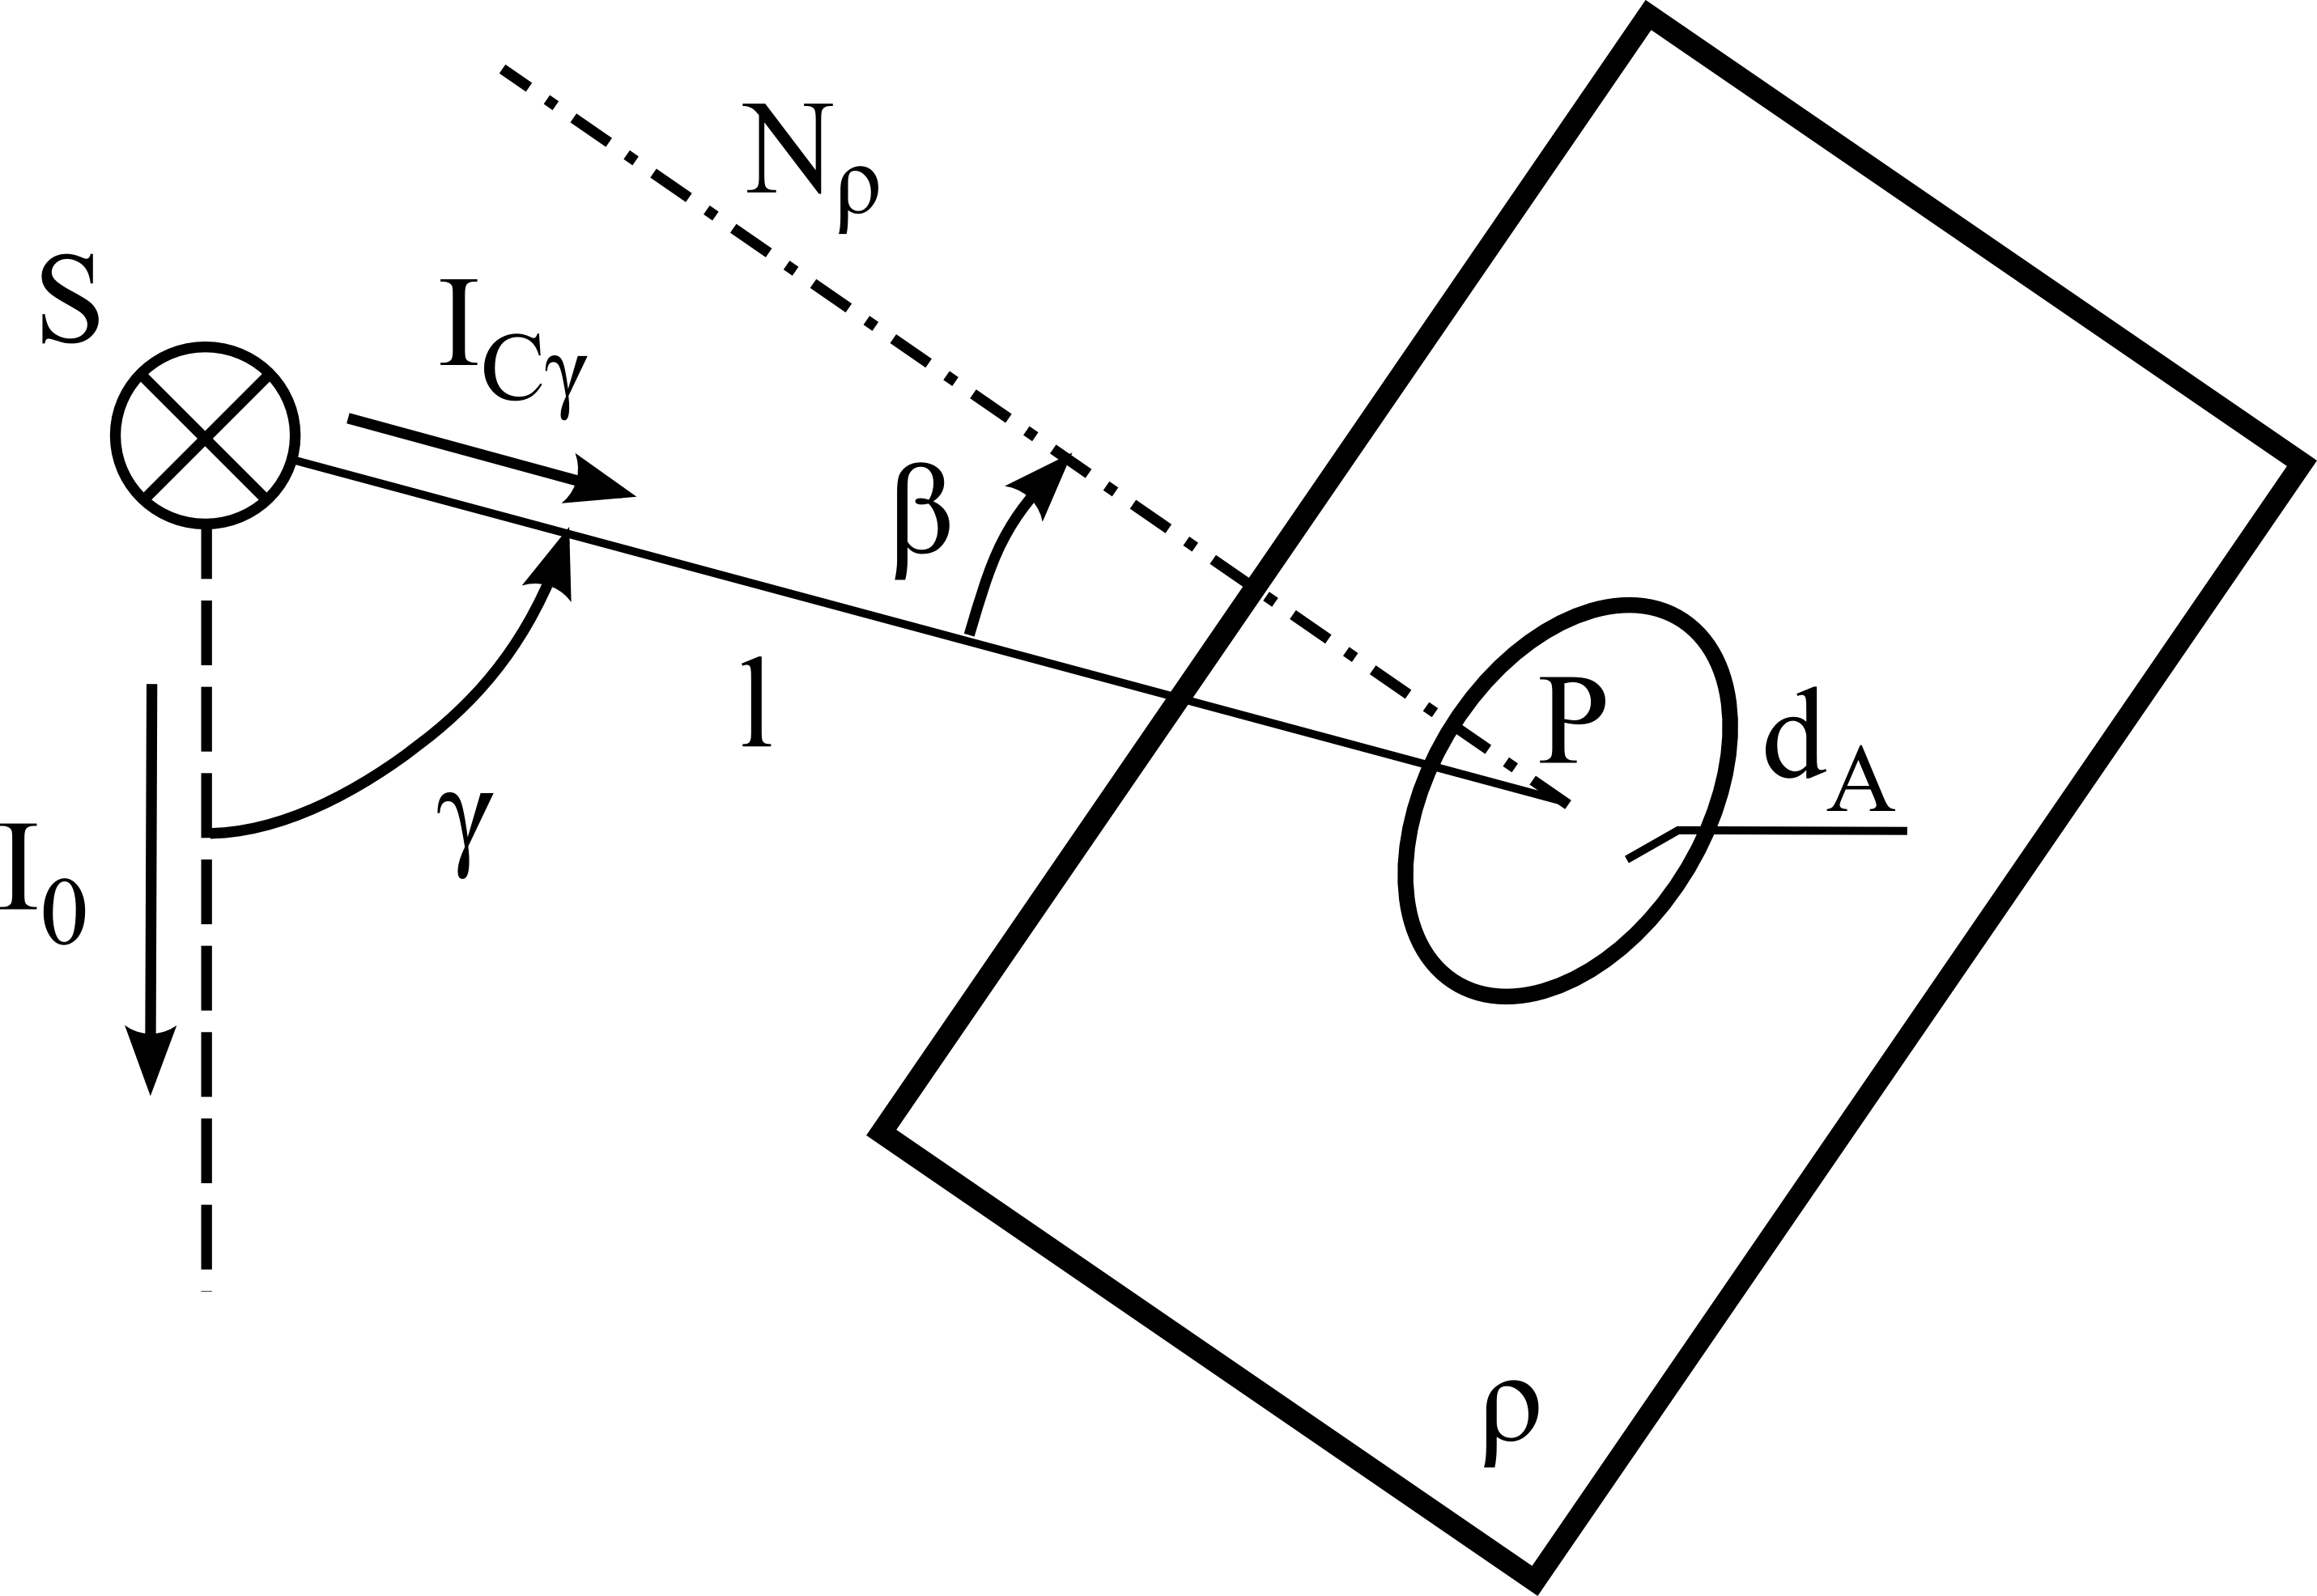
\includegraphics[width=160pt]{315_osvetlenost_bodovym_zdrojem_2}
  \caption{Light source $S$ illuminates point $P$ of plane $\rho$.}
  \label{fig:osv}
\end{figure}

Luminous intensity curves can be found in Eulumdat files of luminaires to enable light scene calculations. Most Eulumdat files of indoor luminaires use the $C-\gamma$ angular coordinate system (Figure~\ref{fig:cgamma}).

\begin{figure}[htb]
  \centering
  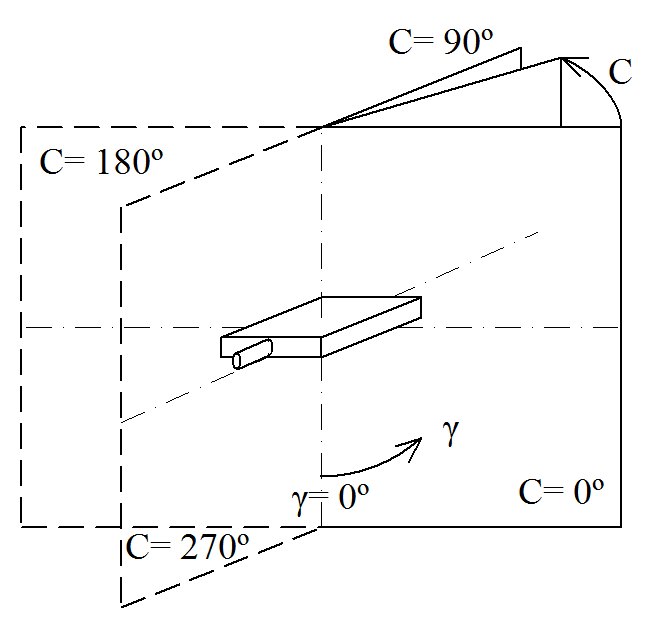
\includegraphics[width=150pt]{Cgama}
  \caption{$C-\gamma$ polar coordinate system with luminaire in center}
  \label{fig:cgamma}
\end{figure}

To bring simulation results closer to real conditions, interaction of light and surfaces has to be included into calculations. Due to the model room's geometric configuration, light reflection affects the light scene the most in this project. Walls, ceiling and floor are becoming secondary light sources after light impact. Using the finite element method, surfaces of the model room are divided into smaller facets each becoming a point light source illuminating other facets leading to multiple reflections (Figure~\ref{fig:difRefl}). During each light reflection a portion of incident luminous flux is absorbed by the surface defined by reflectance value $\rho$. After several reflections the reflected luminous flux becomes negligible.

\begin{figure}[htb]
  \centering
  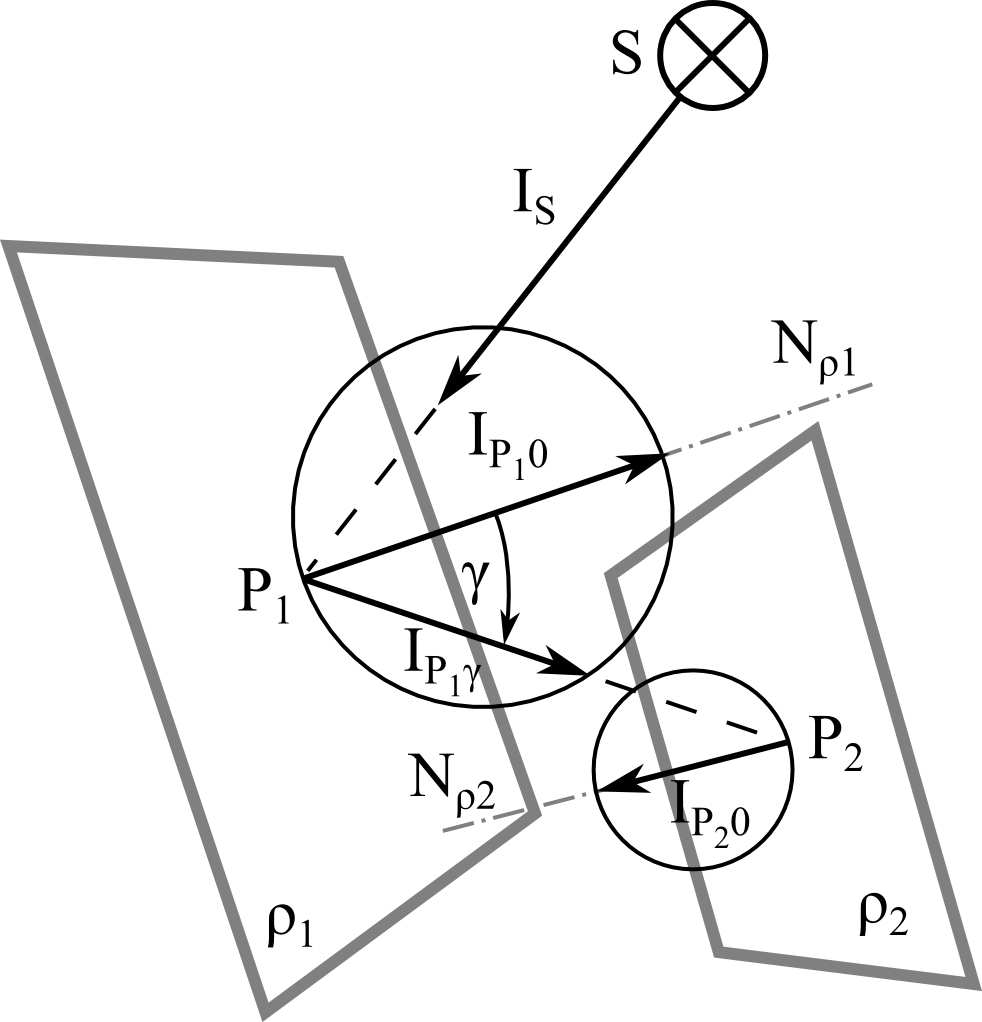
\includegraphics[width=136pt]{diffuseReflection}
  \caption{Multiple reflections between planes $\rho1$ and $\rho2$ with Lambertian reflectance}
  \label{fig:difRefl}
\end{figure}

Most common indoor wall and ceiling surfaces exhibit near Lambertian (diffuse) reflectance. The spatial luminous intensity distribution of purely Lambertian surfaces is dependent only on the referential luminous intensity $I_{0}$ and on angle~$\gamma$ between the surface's normal and the observed direction of the outgoing light ray (Equation~\ref{eq:Igamma}). $I_{0}$ is the luminous intensity of a surface into direction $\gamma=0^{\circ}$, i.e. the surface's normal ($I_{P_{1}0}$ for surface $\rho_1$ and $I_{P_{2}0}$ for surface $\rho_2$ in Figure~\ref{fig:difRefl}). For simplification reasons all surfaces have been chosen to exhibit purely diffuse reflection, including the floor of the model room. Such surfaces become secondary light sources of luminous intensity in direction $\gamma=0^{\circ}$ according to \cite{Habel}:

\begin{equation}
I_{0}=\frac{\rho \cdot E \cdot dA}{\pi} \quad \mathrm{(cd;-,lx,m^{2})}
\label{eq:lumInt}
\end{equation}

where:
\begin{description}
	\item[$I_{0}$] is the referential luminous intensity of the facet in direction of the facet's normal,
	\item[$\rho$] is the facet's integral reflectance,
	\item[$E$] is the facet's illuminance,
	\item[$dA$] is the facet's area.
\end{description}

It must be noted, that luminous intensity is defined only for point light sources. The larger the facet's area $dA$, the lower the calculation accuracy~\cite{handbook}.

After obtaining $I_{0}$, the luminous intensity curve of a facet of Lambertian reflectance will be:

\begin{equation}
I_{\gamma}=I_{0} \cdot \cos(\gamma) \quad \mathrm{(cd;cd,-)}
\label{eq:Igamma}
\end{equation}

where:
\begin{description}
	\item[$I_{\gamma}$] is the luminous intensity in direction $\gamma$.
%	\item[$I_{0}$] is the luminous intensity in direction of facet's normal,
%	\item[$\gamma$] is the angle between the facet's normal and the required direction.
\end{description}

Calculating resulting luminous intensities $I_{0}$ of all available facets of the model room becoming secondary light sources after light impact is achieved in several passes depending on the required amount of reflections. For each facet of the model room light flux cast by primary light sources and the remaining facets is calculated during a single pass. The newly obtained values can then be used later for another pass or for the final reference plane illuminance calculations.

%\begin{itemize}
%	\item Primary light sources emit light incident on visible facets (direct illumination). Initial illuminance $E_{0\rho}$ of facet $\rho$ is obtained by summing up all partial illuminances from all primary light sources (Equation~\ref{eq:illSum}).
%	\item Facets become secondary light sources. Their spacial luminous intensity distributions can be obtained from Equation~\ref{eq:lumInt} and \ref{eq:Igamma} using initial illuminance $E_{0}$. Facet's~$\rho$ illuminance~$E_{1\rho}$ is obtained using Equation~\ref{eq:illSum} and all visible facets as light sources.
%	\item 
%\end{itemize}
%
%First of all primary light sources emit light incident on those facets. Using Equation~\ref{eq:illSum} facets' illuminances can be calculated. 
\section{Model Room Illuminance Calculation}
The algorithm was tested on a model room of dimension 10~m $\times$ 5~m $\times$ 4~m. Any barriers or equipment were not taken into account. Pure diffuse reflections were considered with facets' reflectances:

\begin{itemize}
	\item $\rho = 0.2$ for floor,
	\item $\rho = 0.5$ for walls,
	\item $\rho = 0.7$ for ceiling.
\end{itemize}

Each facet was of dimensions 0.25~m $\times$ 0.25~m. 4~reflections were evaluated for each solution, because a higher count of reflections has little to no effect on the overall results. Furthermore each additional reflection slows down calculations significantly. It was found out that there was an increase of less than 10~\% of the resulting illuminance after the 4\textsuperscript{th} reflection. This fact was tested in a simulation with only a single lamp placed in the middle of the room's ceiling. The result is graphically shown in Figure~\ref{fig:reflDif}.

\begin{figure}[htb]
  \centering
  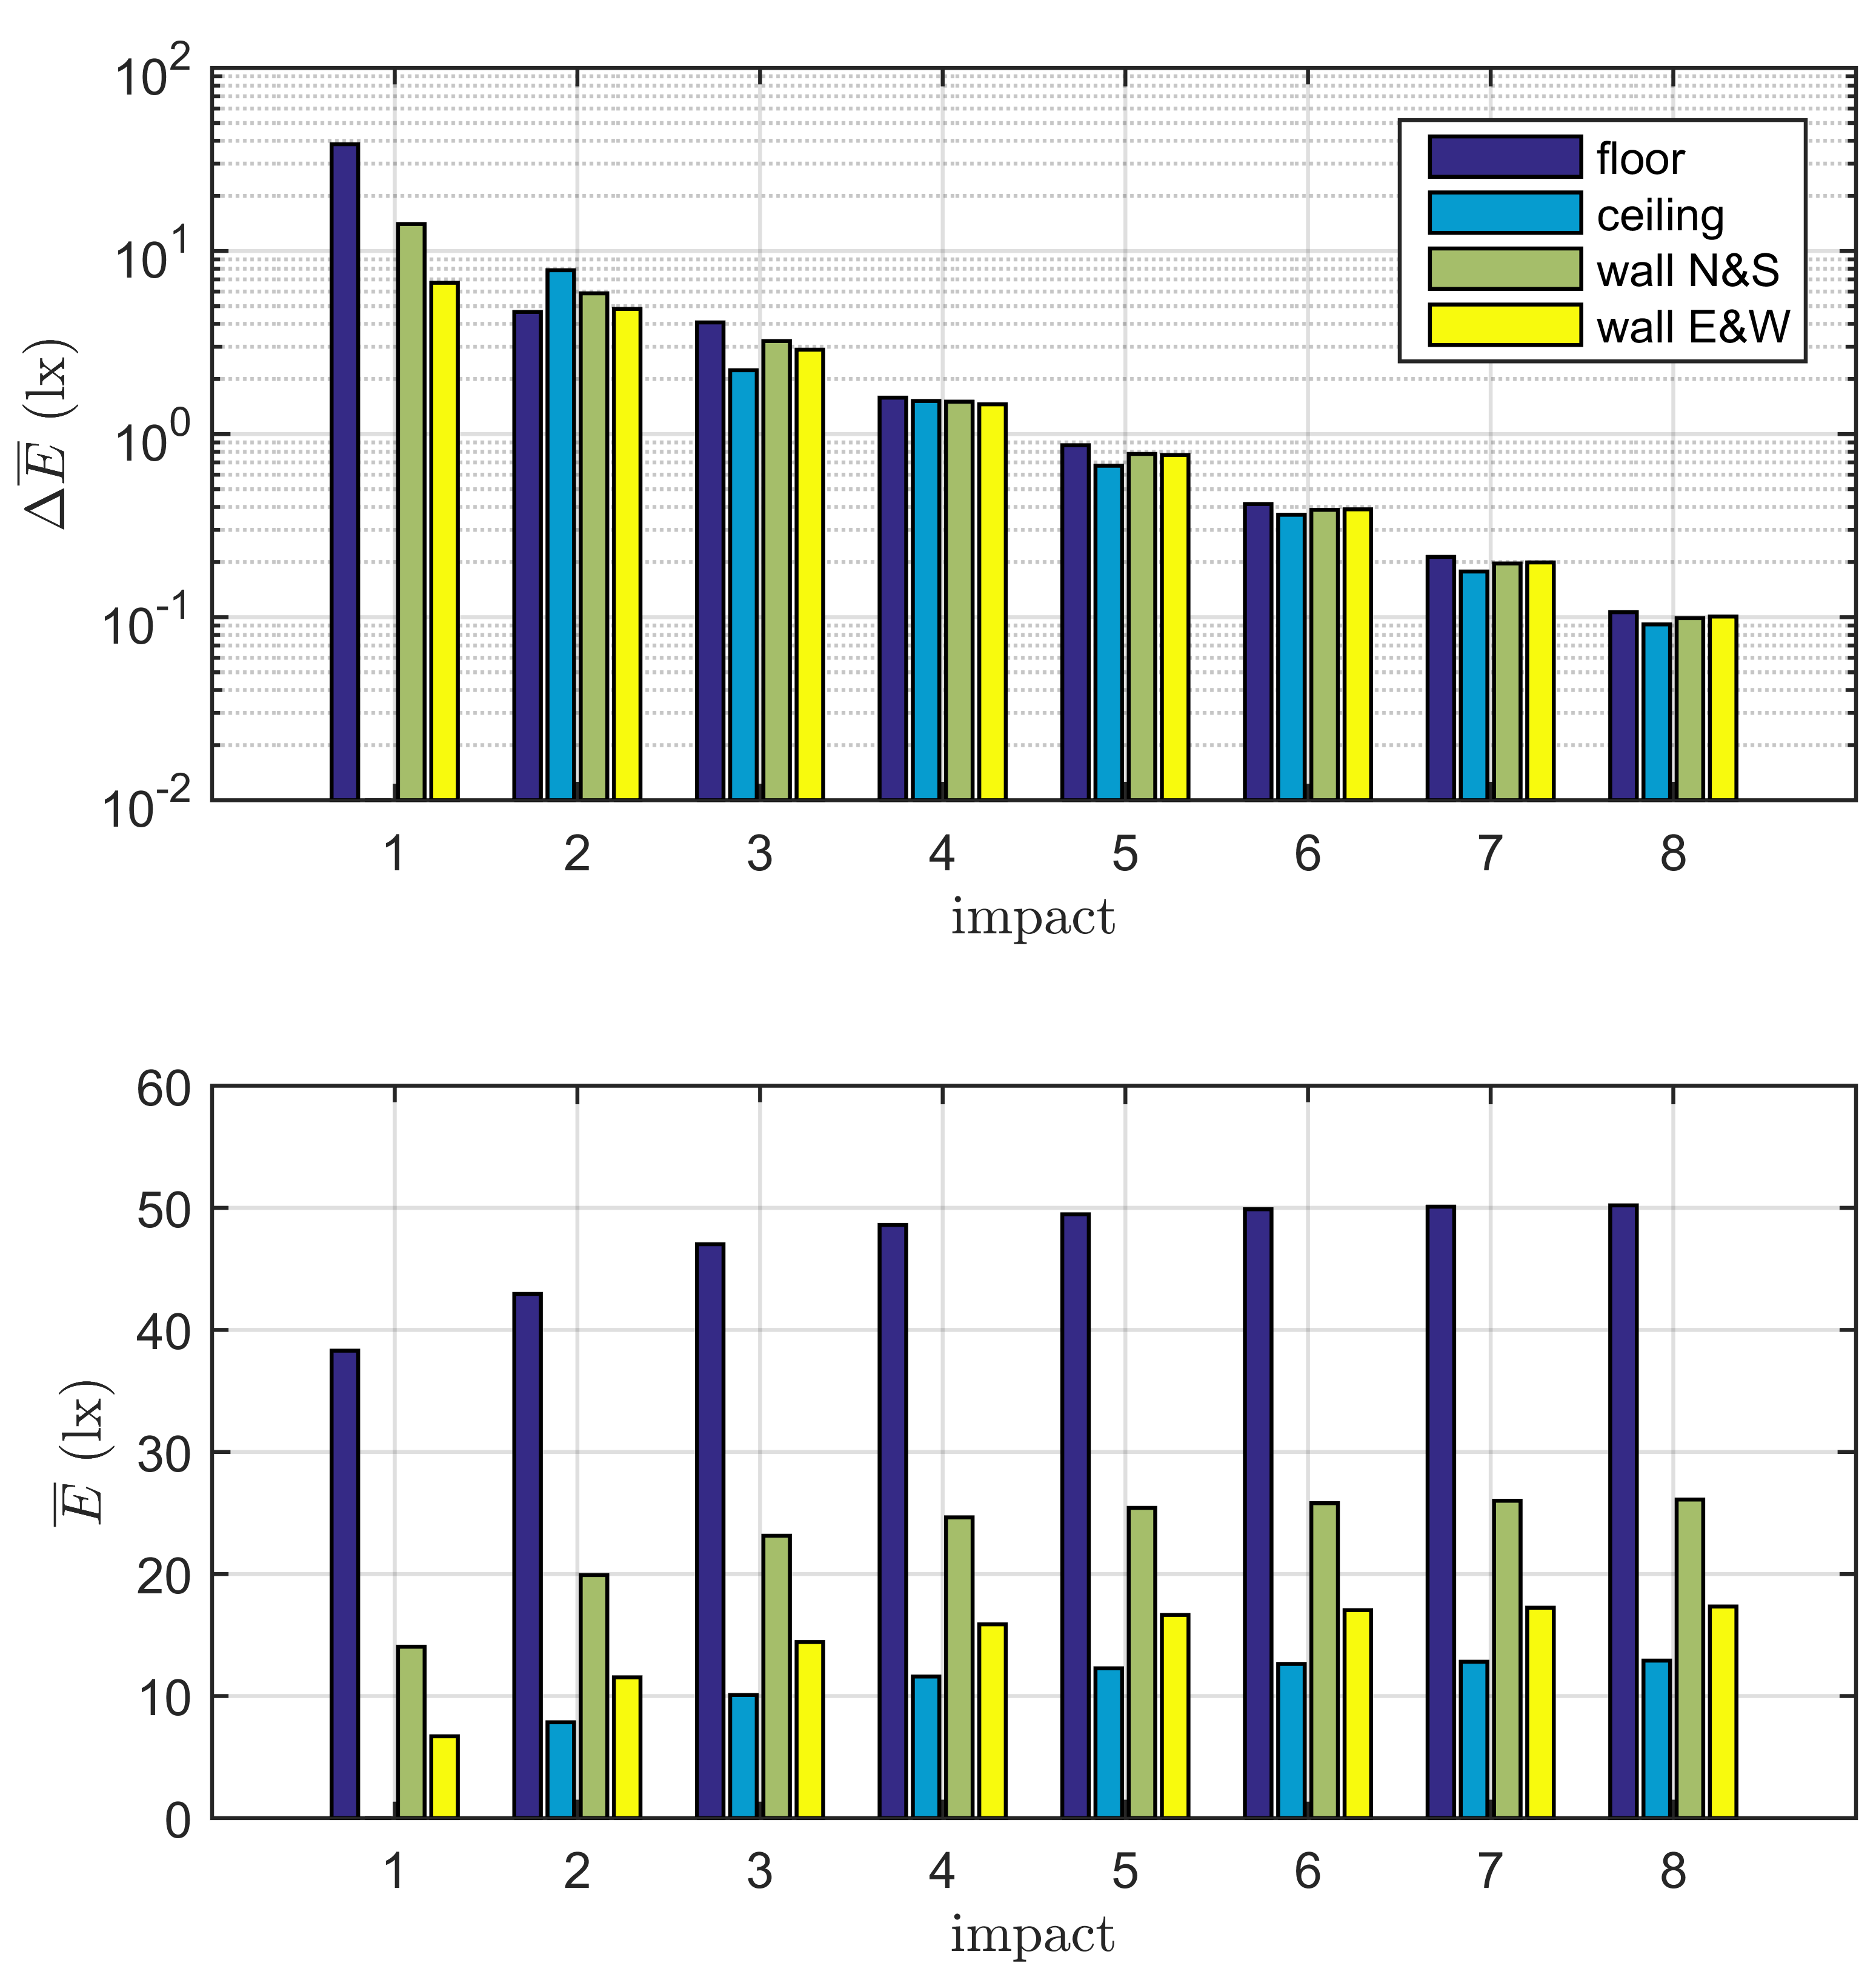
\includegraphics[width=\columnwidth]{reflDif}
  \caption{Increase of the average wall illuminance for one lamp mounted in the center of the room's ceiling depending on the count of light impacts, i.e. number of reflections - 1.}
  \label{fig:reflDif}
\end{figure}

A grid of evenly spaced control points was placed on the reference plane with 25~cm distances between neighboring points. The luminaires were placed in a rectangular area on the ceiling that starts 0.5~m from the E\&W walls and 0.4~m from N\&S walls. All further presented results were evaluated for the same luminaire  MSTR~SLB~4x18W. The luminaire's spacial luminous intensity distribution data were taken from the software "Building Design". All placed luminaires were equally oriented, being described by a normal vector of the $C0^\circ-C180^\circ$ plane in each test parallel with axis $y$ (Figure~\ref{fig:modRoom}). The luminous intensity curve of the used luminaire is shown in Figure~\ref{fig:IDiag}. The considered dimension of the luminaire were 595~mm $\times$ 595~mm $\times$ 80~mm.

\begin{figure}[htb]
  \centering
  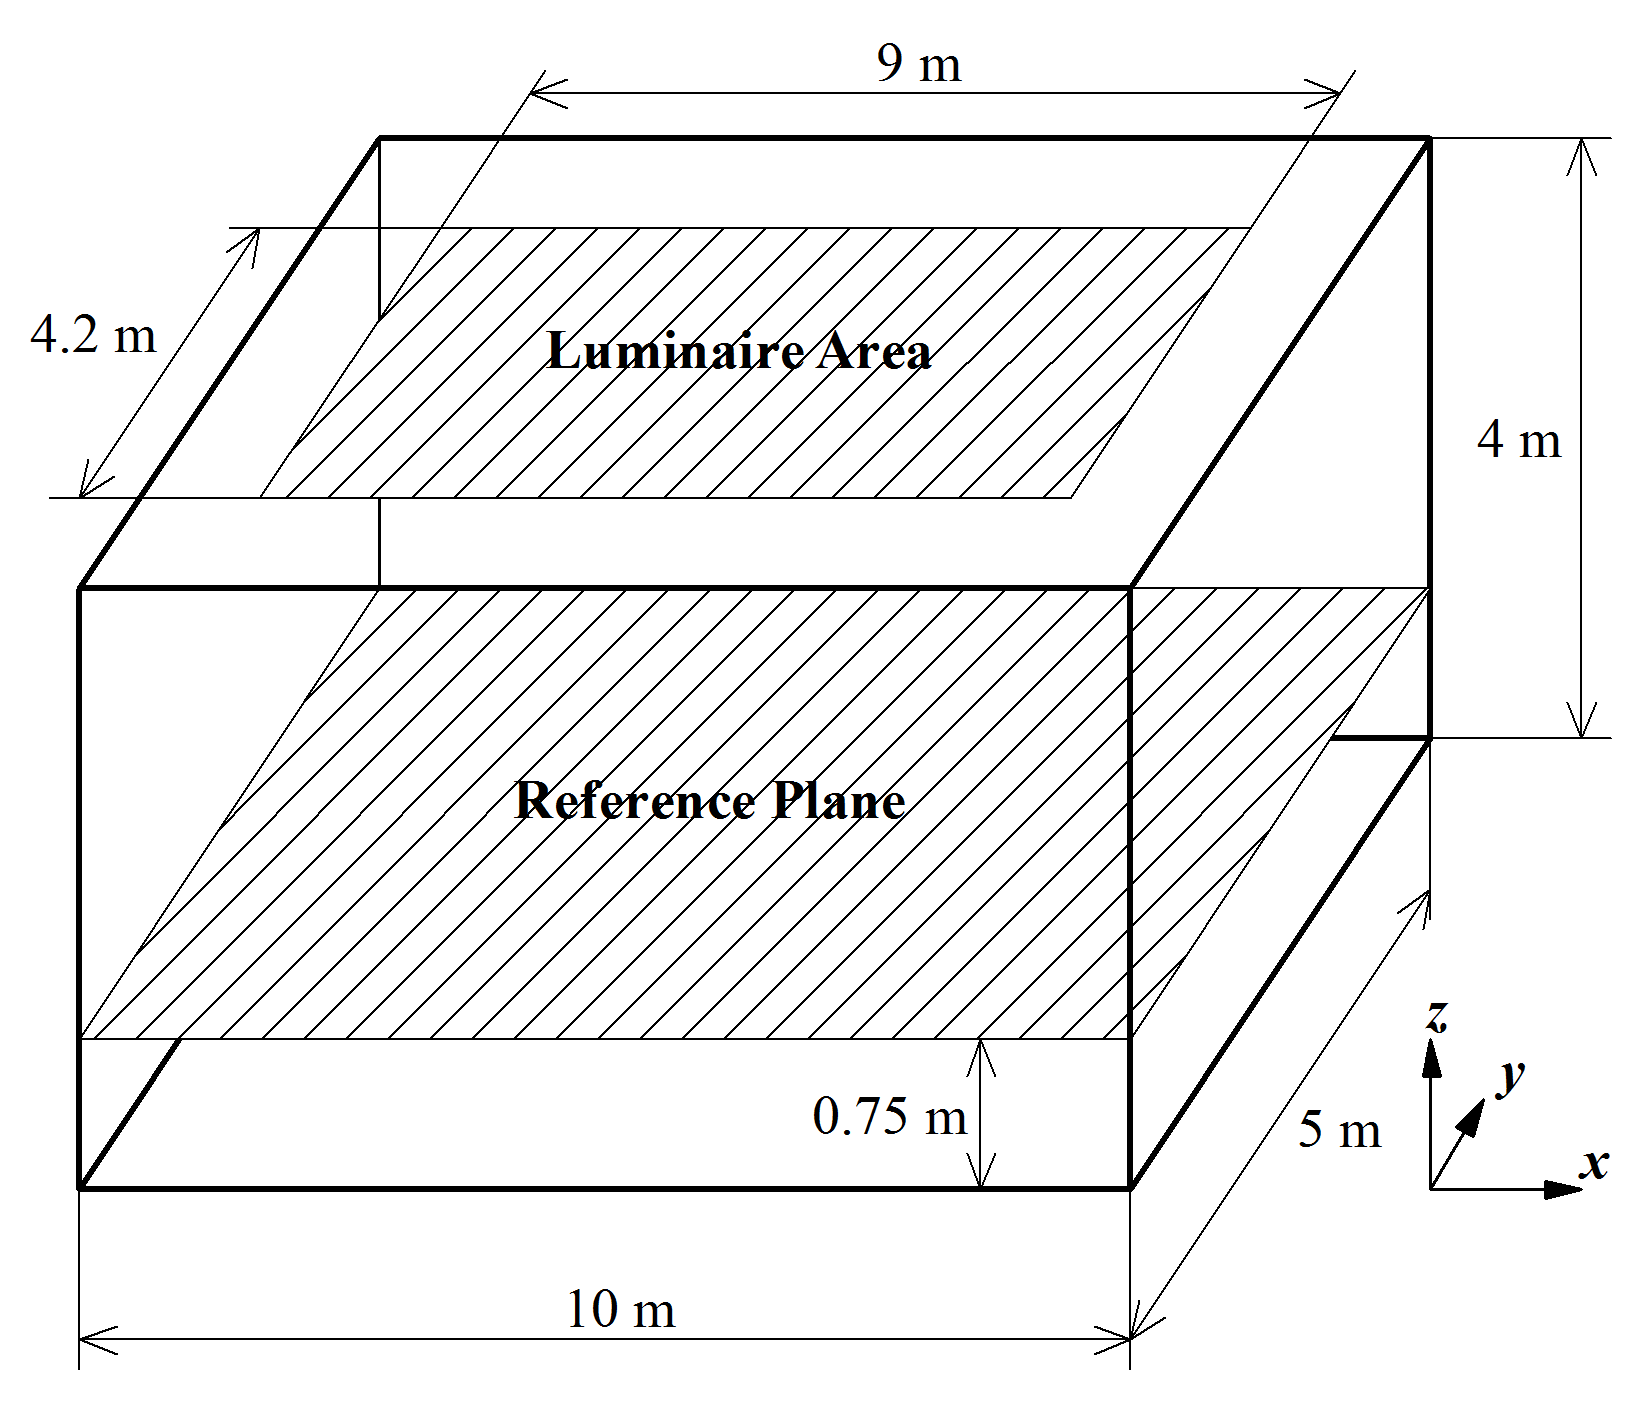
\includegraphics[width=\columnwidth]{modRoom}
  \caption{Model room dimensions}
  \label{fig:modRoom}
\end{figure}

\begin{figure}[htb]
  \centering
  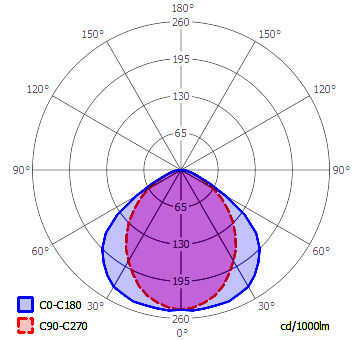
\includegraphics[width=0.8\columnwidth]{IDiag}
  \caption{Luminous intensity distribution curve of the luminaire MSTR SLB 4x18W}
  \label{fig:IDiag}
\end{figure}
\section{Genetic Algorithm Introduction}
The genetic algorithms (GA) are the part of the evolutionary computing. Similar to the living organism are the solutions represented by their genotype, that represents the parameter coding and by phenotype, that represents behaviour, response and features of the solutions. The genotype is typically coded as a vector of parameters termed a chromosome, with elements being described as genes~\cite{Fogel2006}. Each solution is considered according to its phenotype and selected if the phenotype fits the constraints and conditions of an examined environment or task. The ability to survive and reproduce in specific environment is called fitness. The Selection must maintain or increase the fitness of solution sets that are called populations. Each set of solutions corresponds to one so called generation.

Each generation starts with selecting solutions with high fitness to form set of parent solutions for the next population. After that the process of crossovers and mutations creates new population. The crossover combines two chromosomes of parent solutions together. The one-point crossover was used in presented solutions. Parent chromosomes are randomly split at the same point and the parts that follow that point are exchanged. The mutation changes the chromosome directly. It can change the value of a selected gene for example. The paper deals with the implemented mutation in the next section. Both the crossovers and mutations are made only with certain probability. The probability of crossovers is typically high (more than 90~\%) in comparison to mutation, which must be low (under 10~\%). High probability of mutation makes the optimization difficult because of the high rate of change in chromosomes.

\section{Design Requirements}
The design results must involve all requirements given by standards. Therefore the first task is always to obtain at least the minimal level of illuminance and uniformity. It is obvious that several designs overpass the minimal values and fit the standard. Better specification and other restrictions for the results must be done. Some specifications arise from the designer's preferences. The solutions with higher efficiency are the better for example. Other examples of designer's preferences can involve:

\begin{enumerate}
	\item[(i)] the minimal count of luminaires (efficiency),
	\item[(ii)] symmetry of the luminaires placement,
	\item[(iii)] the placement restricted only in specific area,
	\item[(iv)] placement in specific shape of groups of luminaires,
	\item[(v)] get the highest illuminance for given uniformity etc.
\end{enumerate}

The result must also respect the luminaires dimensions. Proximity among luminaires can be unfeasible.

The genetic algorithm can handle the requirements in two ways. First introduces the requirements as a part of the fitness function. It is the case, where the requirements are some part of the phenotype. This is very common and it can be used for example in case of target illuminance and uniformity accomplishment. Other specification fitting this method are the (i) and (v) from the list above. The usage will be described in the next section. 

Some requirements are very difficult to introduce in the fitness function. Therefore the second possible way uses the restrictions in the space of allowed solutions. Such method fits the specification (ii), (iii) and (iv) from the list above.
\section{Fitness Function}
The fitness function is the essential part of the GA that assesses the solutions. The target solution's fitness function value is the minimum or maximum of the fitness function, depending on the fitness function design. There are no general rules for its range of values and only simple recommendations for its creation. The target value of average maintained illuminance and of uniformity are watched by the algorithm. The output design is the most effective after the target values are reached with minimum count of luminaires. Therefore the minimization of the luminaires count is also expected.

The first attempt to create a suitable fitness function was based on the idea, that the minimum luminaire number would be obtained just by the requirement of a target illuminance. The algorithm was supposed to reach the target value of illuminance with the highest possible uniformity. However only the restriction of getting the exact value of the illuminance was not sufficient to get the minimum count of luminaires. The demand to maximize uniformity favored solutions with little bit more luminaires than needed to fulfill the minimum illuminance requirement. Therefore the minimalization of luminaire count had to be directly included into the fitness function.

The fitness function bellow is currently used in the algorithm. Solutions that do not reach basic requirements of target illuminance or uniformity are evaluated by length of the chromosome $L$ (Equation~\ref{eq:chromLength}):

\begin{equation}
\label{eq:fitV2EUA}
	f\left(C,\overline{E}_{m}, U_0\right)= L
\end{equation}

\noindent Otherwise the fitness is evaluated by:

\begin{equation}
\label{eq:fitV2EUB}
\begin{split}
f\left(C, \overline{E}_{m}, U_0\right)&=C +\\
& + \left( 1 - \alpha\right)\cdot\frac{\overline{E}_{mT}}{\overline{E}_{m}+\epsilon} + \\
& + \alpha\cdot\frac{U_{0T}}{U_0 + \epsilon}
\end{split}
\end{equation}

\noindent where:
\begin{description}
	\item[$C$] is the count of luminaires,
	\item[$\overline{E}_{m}$] is the calculated maintained average value of illuminance,
	\item[$\overline{E}_{mT}$] is the target maintained average value of illuminance,
	\item[$U_0$] is the calculated lighting uniformity,
	\item[$U_{0T}$] is the target lighting uniformity,
	\item[$\alpha$] is a number between 0 and 1,
	\item[$\epsilon$] is a very small number, that prevents the division by 0.
\end{description}

$\alpha$ represents the designer's intention to prefer one of the parameter to another. The target ratio between relative values of the parameters can be obtained from partial derivation of the fitness function:

\begin{equation}
\label{eq:fitV2ratio}
R =\frac{\overline{E}_{m}}{\overline{E}_{mT}}\cdot\frac{U_{0T}}{U_0}=\sqrt{\frac{1-\alpha}{\alpha}}
\end{equation}

\noindent There is no preference if $\alpha$ is equal to $0.5$. Only illuminance is considered for $\alpha = 0$ and only uniformity is considered for $\alpha = 1$.

This fitness function is supposed to be minimized, i.e. the smaller the output of the fitness function, the higher the quality of the solution. Equation \ref{eq:fitV2EUB} can be, if close to the target values of illuminance and uniformity, separated into an integer part, given only by the count of luminaires $h_1\left(C\right)= C$ and a fraction part that is given by:

\begin{equation}
\label{eq:fitV2frac}
	h_2\left(\overline{E}_{m}, U_0\right)= \left( 1 - \alpha\right)\cdot\frac{\overline{E}_{mT}}{\overline{E}_{m}+\epsilon} + \alpha\cdot\frac{U_{0T}}{U_0 + \epsilon}
\end{equation}

The main impact of the integer part $h_1\left(C\right)$ occurs at the beginning of the optimization. Only solutions that fulfill the standard requirements can have a smaller value of fitness than the length of its chromosome. For other solutions the most effective way to minimize the outcome of Equation~\ref{eq:fitV2EUB} is by decreasing the count of luminaires. Changes of part $h_2\left(\overline{E}_{m}, U_0\right)$ are less significant, because for high counts of luminaires, the denominator of Equation~\ref{eq:fitV2frac} is much higher than the numerator. Therefore the resulting fraction is very small.

After getting the optimal count of luminaires, function's $h_2\left(\overline{E}_{m}, U_0\right)$ output value will be close to 1 but smaller. An effective way to minimize Equation~\ref{eq:fitV2EUB} is to get the highest possible illuminance and uniformity for the given number of luminaires.

The defined fitness function was used for several runs of the GA and has always worked well. However there is a known problem in the definition of Equation~\ref{eq:fitV2EUA}. Consider the case, that none of the initial solutions would fulfill the standard requirements. Then all of them would have the same fitness value equal to chromosome length $L$. It is very probable, that after selection, crossovers and mutations at least a single solution will appear fulfilling the standard requirements. But there can also be rare cases, in which the algorithm never optimizes the count of luminaires, because the fitness function in these cases is independent on all parameters of their solutions. The presence of the problem is more probable for very small population sizes, small count of generations, small probability of mutations or for an inappropriately designed selection method.

Some parameter dependency ca be added to Equation~\ref{eq:fitV2EUA}. However it was quite useless for the further described settings of the GA and the chosen selection method. It would be extremely rare if any of the solutions fulfilling the standard requirements would not appear after a couple of generations.

\section{GA Outputs}

\subsection{Settings}

\subsection{Symmetry Comparison}

\subsection{Different Preferences}

\subsection{No Reflection from South Wall}
\section{Conclusion}

The presented GA was tested for several types of luminaires. It seemed to be a quite good tool for placement design and comparison optimized results dependent on luminare type. The main disadvantage of the method is long time of evaluation.

The output designs little differ for the same settings. Similar outputs are got especially for the mirror symmetry. However basic features of the design are always obvious. The luminaires are located closer together in case of prefered illuminance in comparison to prefered uniformity.

It is obvious from presented results that considering reflections has important role in the design. The reflections change the resulting illuminance and uniformity and clearly affect the placement.

The next stage of the project supposes to use the same algorithm for solution of different shapes of rooms including some room equipment. The Algorithm considering not diffused reflections is in progress too.

\newpage

\begin{thebibliography}{99}

\bibitem{12464}
\v{C}SN EN 12464-1. \textit{Sv\v{e}tlo a osv\v{e}tlen\'{i} - Osv\v{e}tlen\'{i} pracovn\'{i}ch prostor\r{u}: \v{C}\'{a}st 1: Vnit\v{r}n\'{i} pracovn\'{i} prostory.} Praha: \'{U}\v{r}ad pro technickou normalizaci, metrologii a st\'{a}tn\'{i} zku\v{s}ebnictv\'{i}, 2012

\bibitem{360011}
\v{C}SN 36 0011-1. \textit{M\v{e}\v{r}en\'{i} osv\v{e}tlen\'{i} vnit\v{r}n\'{i}ch prostor\r{u}: \v{C}\'{a}st 1: Z\'{a}kladn\'{i} ustanoven\'{i}}. Praha: \v{C}esk\'{i} normaliza\v{c}n\'{i} institut, 2006.


\bibitem{12665}
\v{C}SN EN 12665. \textit{Sv\v{e}tlo a osv\v{e}tlen\'{i} - Z\'{a}kladn\'{i} term\'{i}ny a krit\'{e}ria pro stanoven\'{i} po\v{z}adavk\r{u} na osv\v{e}tlen\'{i}}. Praha: \'{U}\v{r}ad pro technickou normalizaci, metrologii a st\'{a}tn\'{i} zku\v{s}ebnictv\'{i}, 2012.

\bibitem{CIE97}
INTERNATIONAL COMMISSION ON ILLUMINATION.\textit{ CIE 97: 2005, Guide on the maintenance of indoor electric lighting systems.} 2nd~ed. Vienna: CIE, 2005. ISBN 9783901906459.

\bibitem{Habel} 
J. Habel. \textit{Sv\v{e}tlo a osv\v{e}tlov\'{a}n\'{i}}. Praha: FCC Public, 2013, 622~s. ISBN 978-80-86534-21-3.

\bibitem{Fogel2006}
D. B. Fogel. \textit{Evolutionary computation: toward a new philosophy of machine intelligence}. 3rd ed. Hoboken: John Wiley, 2006, xvii, 274~s. ISBN 04-716-6951-2.

\end{thebibliography}

\end{document}
